% Homework-4.tex's last substantial revision: 2023-03-18 10:50 EST
% Template.tex's last substantial revision: 2023-03-09 10:29 EST
% "Substantial" for Template.tex is laxer than for content-ful .texs
% Revision contents: add white/weaker QED


%%%%%%%%%%%%%%%%%%%%%%%%%%%%%%%%%%%%%%%%%%%%%%%%%%%%%%%%%%%%%%%%%%%%%%%%%%%%%%%%
% MANAGE PDFs FOR SCREEN-READING %%%%%%%%%%%%%%%%%%%%%%%%%%%%%%%%%%%%%%%%%%%%%%%
%%%%%%%%%%%%%%%%%%%%%%%%%%%%%%%%%%%%%%%%%%%%%%%%%%%%%%%%%%%%%%%%%%%%%%%%%%%%%%%%
%\RequirePackage{pdfmanagement-testphase} % TK Uncomment when dependencies gotten
%\DeclareDocumentMetadata{uncompress,pdfversion=2.0} % TK uncomment when control sequence done
% See: TK idk find the url



%%%%%%%%%%%%%%%%%%%%%%%%%%%%%%%%%%%%%%%%%%%%%%%%%%%%%%%%%%%%%%%%%%%%%%%%%%%%%%%%
% TK LINKS (INSPIRATION) %%%%%%%%%%%%%%%%%%%%%%%%%%%%%%%%%%%%%%%%%%%%%%
%%%%%%%%%%%%%%%%%%%%%%%%%%%%%%%%%%%%%%%%%%%%%%%%%%%%%%%%%%%%%%%%%%%%%%%%%%%%%%%%
% `standalone` package: put pictures etc. into own source files
% for header/footer: https://tex.stackexchange.com/a/203059
% for info about draft mode: https://tex.stackexchange.com/q/49277



%%%%%%%%%%%%%%%%%%%%%%%%%%%%%%%%%%%%%%%%%%%%%%%%%%%%%%%%%%%%%%%%%%%%%%%%%%%%%%%%
% TK LINKS (GUIDES) %%%%%%%%%%%%%%%%%%%%%%%%%%%%%%%%%%%%%%%%%%%%%%%%%%%%%%%%%%%%
%%%%%%%%%%%%%%%%%%%%%%%%%%%%%%%%%%%%%%%%%%%%%%%%%%%%%%%%%%%%%%%%%%%%%%%%%%%%%%%%
% Proofwiki House Style: https://proofwiki.org/wiki/Help:Editing/House_Style
% Typography in general: https://practicaltypography.com/summary-of-key-rules.html
% LaTeX mistakes (see also comments): http://www.johndcook.com/blog/2010/02/15/top-latex-mistakes/
% best practices for templating: https://tex.stackexchange.com/questions/40760/best-practice-on-organising-your-preamble
% .dtx tutorial: https://www.ctan.org/tex-archive/info/dtxtut
% standalone and .fmts: https://tex.stackexchange.com/questions/42414/using-the-standalone-package-with-a-fmt-file
% why put title+metadata before hyperref?: https://tex.stackexchange.com/questions/17218/make-hyperref-take-pdfinfo-from-title-and-author
% for fixing vscode/latex workshop pdf viewer: https://tex.stackexchange.com/questions/527463/pdf-preview-in-visual-studio-code
% for CV: https://latex-tutorial.com/cv-latex-guide/
% inspo for templating: https://tex.stackexchange.com/q/59702
% for making captions of minteds: https://tex.stackexchange.com/a/305392
% for speeding up TikZ: https://tex.stackexchange.com/q/45
% for improving minteds: https://latex-tutorial.com/code-listings/
% for highlighting code (colored boxes) on top of syntax highlighting: https://tex.stackexchange.com/a/49309



%%%%%%%%%%%%%%%%%%%%%%%%%%%%%%%%%%%%%%%%%%%%%%%%%%%%%%%%%%%%%%%%%%%%%%%%%%%%%%%%
% TK TODO %%%%%%%%%%%%%%%%%%%%%%%%%%%%%%%%%%%%%%%%%%%%%%%%%%%%%%%%%%%%%%%%%%%%%%
%%%%%%%%%%%%%%%%%%%%%%%%%%%%%%%%%%%%%%%%%%%%%%%%%%%%%%%%%%%%%%%%%%%%%%%%%%%%%%%%
%
% Document-level
% - make separate latex file to preload preamble
% - make separate latex file as my design ethos manifesto
%
% Component-level
% - \textbf{Show}case other things (e.g. codeblocks, highlighting, qeding)
% - make remarks and proof? blocks (tcolorbox)
%
% Text-level
% - override \Vec (`asmmath`?) command with my own
% - fix vertical spacing between Comment and math
% - directional (from NW, bend, to W) arrows for proof comments (first instance)
% ✅ align 2nd level enumeration items with 1st level (ask on stackexchange)
% --- create "CSCI-2725" enum environment to handle this
% --- solution (in question): https://tex.stackexchange.com/q/419352/
% - fix square root sign stroke thickness (too thick) in single-$/text-math mode
% ✅ center (align*) equations in prompt in various problems (enumerate)
% --- solution (2nd part of ans.): https://tex.stackexchange.com/a/54686/
% --- other solution (more flexible but needs multiple compilation): https://tex.stackexchange.com/a/9640/
%
% Comment-level
% - switch "See" to "Credit" appropriately



%%%%%%%%%%%%%%%%%%%%%%%%%%%%%%%%%%%%%%%%%%%%%%%%%%%%%%%%%%%%%%%%%%%%%%%%%%%%%%%%
% CLASS %%%%%%%%%%%%%%%%%%%%%%%%%%%%%%%%%%%%%%%%%%%%%%%%%%%%%%%%%%%%%%%%%%%%%%%%
%%%%%%%%%%%%%%%%%%%%%%%%%%%%%%%%%%%%%%%%%%%%%%%%%%%%%%%%%%%%%%%%%%%%%%%%%%%%%%%%
\documentclass[12pt, a4paper]{article}



%%%%%%%%%%%%%%%%%%%%%%%%%%%%%%%%%%%%%%%%%%%%%%%%%%%%%%%%%%%%%%%%%%%%%%%%%%%%%%%%
% FONTS and ENCODING %%%%%%%%%%%%%%%%%%%%%%%%%%%%%%%%%%%%%%%%%%%%%%%%%%%%%%%%%%%
%%%%%%%%%%%%%%%%%%%%%%%%%%%%%%%%%%%%%%%%%%%%%%%%%%%%%%%%%%%%%%%%%%%%%%%%%%%%%%%%
%
% See: https://tex.stackexchange.com/q/59702
\usepackage[utf8]{inputenc}	      % allows input of accented characters directly from the keyboard
							              			% https://tex.stackexchange.com/questions/44694/fontenc-vs-inputenc
%
\usepackage{libertine}						% Linux Libertine (text) font family
\usepackage[libertine,						% math-mode fonts to harmonize with Libertine text fonts.
smallerops, varg, cmbraces, noamssymbols, ]{newtxmath}
                                  % [libertine] = substitutes libertine for Times
                                  % [smallerops] = smaller \sum,etc.
                                  % [varg] = distinctive math letters
                                  % [cmbraces] = thicker braces
                                  % [noamssymbols] = prevent TXAMSadd from loading
\let\Bbbk\relax										% disables newtxmath's definition of \Bbbk in favor of amssymb's (blackboard bold lowercase k)
                                  % This choice of disabling is arbitrary.
                                  % See: https://tex.stackexchange.com/a/587033
%\usepackage{newtxtext}		  		  % loads clones of reasonably well-match fonts (Helvetica and a monospaced)
%\usepackage{newpxtext,newpxmath} % based on Zapf's Palatino font
%
\usepackage{microtype}						% to break monospace (texttt) lines correctly
% the below does not work with ragged-right env. (leave disabled to stop warnings)
%\usepackage[htt]{hyphenat}       % to hyphenate monospace (texttt) lines correctly
							              			% See: https://tex.stackexchange.com/a/10378
\usepackage[T1]{fontenc} 	        % ensures proper hyphenation
																																	% why load after non-CM fonts?: https://tex.stackexchange.com/a/2869



%%%%%%%%%%%%%%%%%%%%%%%%%%%%%%%%%%%%%%%%%%%%%%%%%%%%%%%%%%%%%%%%%%%%%%%%%%%%%%%%
% AMS MATH %%%%%%%%%%%%%%%%%%%%%%%%%%%%%%%%%%%%%%%%%%%%%%%%%%%%%%%%%%%%%%%%%%%%%
%%%%%%%%%%%%%%%%%%%%%%%%%%%%%%%%%%%%%%%%%%%%%%%%%%%%%%%%%%%%%%%%%%%%%%%%%%%%%%%%
% \usepackage{amsmath}      % loads amstext, amsbsy, amsopn but not amssymb
                            % equation stuff (eqref, subequations, equation, align, gather, flalign, multline, alignat, split...)
                            % redundant by newtxmath
% \usepackage{amsfonts}     % may be redundant with amsmath
\usepackage{amssymb}        % may be redundant with amsmath (enable for \therefore)
% \numberwithin{equation}{section}  % reset equation counters at start of each "section" and prefix numbers by section number
% \numberwithin{figure}{section}    % reset figure   counters at start of each "section" and prefix numbers by section number



%%%%%%%%%%%%%%%%%%%%%%%%%%%%%%%%%%%%%%%%%%%%%%%%%%%%%%%%%%%%%%%%%%%%%%%%%%%%%%%%
% LAYOUT %%%%%%%%%%%%%%%%%%%%%%%%%%%%%%%%%%%%%%%%%%%%%%%%%%%%%%%%%%%%%%%%%%%%%%%
%%%%%%%%%%%%%%%%%%%%%%%%%%%%%%%%%%%%%%%%%%%%%%%%%%%%%%%%%%%%%%%%%%%%%%%%%%%%%%%%
%
% force ~71 (65) characters per line
% Credit: https://tex.stackexchange.com/a/59636
\usepackage{geometry}
\newlength{\alphabet}
\settowidth{\alphabet}{\normalfont abcdefghijklmnopqrstuvwxyz}
\geometry{textwidth = 2.75\alphabet}		% (Note: 2.75 * 26 = 71.5)
% wider for math-heavy, narrower for text-heavy
\makeatletter
\if@twoside
  \geometry{hmarginratio = {2:3}}
\else
  \geometry{hmarginratio = {1:1}}
\fi
\makeatother
%
%
\linespread{1.25}
%
% remove spaces around align (and other display math) envs
% Credit: https://tex.stackexchange.com/a/47403
%\usepackage{etoolbox}
%\newcommand{\zerodisplayskips}{%
%  \setlength{\abovedisplayskip}{12pt}%
%  \setlength{\belowdisplayskip}{12pt}%
%% "short skip" refers to when the text line above/below the display math
%% --ENDS (horizontally) before the display math BEGINS (horizontally)
%% --so the math is raised a bit (vertically) to not leave so much whitespace.
%% --See: https://tex.stackexchange.com/a/30913
%  \setlength{\abovedisplayshortskip}{5pt}%
%  \setlength{\belowdisplayshortskip}{5pt}}
%\appto{\normalsize}{\zerodisplayskips}
%\appto{\small}{\zerodisplayskips}
%\appto{\footnotesize}{\zerodisplayskips}
%



%%%%%%%%%%%%%%%%%%%%%%%%%%%%%%%%%%%%%%%%%%%%%%%%%%%%%%%%%%%%%%%%%%%%%%%%%%%%%%%%
% OTHER PACKAGES %%%%%%%%%%%%%%%%%%%%%%%%%%%%%%%%%%%%%%%%%%%%%%%%%%%%%%%%%%%%%%%
%%%%%%%%%%%%%%%%%%%%%%%%%%%%%%%%%%%%%%%%%%%%%%%%%%%%%%%%%%%%%%%%%%%%%%%%%%%%%%%%
\usepackage{enumitem}
\usepackage{mathtools}				% for multlined, dcases environment
\usepackage{lipsum}						% to fill in with arbitrary text
%\usepackage{datetime2}				% to display \currenttime in \date
%
\usepackage{ntheorem}
\newtheorem{theorem}{Theorem}
%
\usepackage{tcolorbox}				% currently, idk
\tcbuselibrary{most}					% currently, only for Highlight
\usepackage{fancybox}         % for text boxes such as those surrounding \Comments
%
\usepackage{derivative}			  % for upright "d"s and all sorts of derivatives
\usepackage{bm}										% bold math symbols (like vectors)

\usepackage{color}
\definecolor{warm}{HTML}{FFEEBB} % for a warm page background color



%%%%%%%%%%%%%%%%%%%%%%%%%%%%%%%%%%%%%%%%%%%%%%%%%%%%%%%%%%%%%%%%%%%%%%%%%%%%%%%%
% GRAPHICX %%%%%%%%%%%%%%%%%%%%%%%%%%%%%%%%%%%%%%%%%%%%%%%%%%%%%%%%%%%%%%%%%%%%%
%%%%%%%%%%%%%%%%%%%%%%%%%%%%%%%%%%%%%%%%%%%%%%%%%%%%%%%%%%%%%%%%%%%%%%%%%%%%%%%%
\usepackage{graphicx} 		            % options = [final]  = all graphics displayed, regardless of draft option in class
                                      % ^[final] does option clash
                                      % options = [pdftex] = necessary (?) if import PDF files
                                      % no option : when importing ps- and eps-files (?)
\usepackage[export]{adjustbox}
\graphicspath{ {./images/} }  	  		% tell LaTeX where to look for images
% \DeclareGraphicsExtensions{.pdf, .PDF, .jpg, .JPG, .jpeg, .JPEG, .png, .PNG, .bmp, .BMP, .eps, .ps}
\usepackage{float}				            % Improved interface for floating objects; add [H] option
\usepackage{subcaption}		            % allows subfigures (inside figure envs)



%%%%%%%%%%%%%%%%%%%%%%%%%%%%%%%%%%%%%%%%%%%%%%%%%%%%%%%%%%%%%%%%%%%%%%%%%%%%%%%%
% HYPERREF (last) then HYPCAP %%%%%%%%%%%%%%%%%%%%%%%%%%%%%%%%%%%%%%%%%%%%%%%%%%
%%%%%%%%%%%%%%%%%%%%%%%%%%%%%%%%%%%%%%%%%%%%%%%%%%%%%%%%%%%%%%%%%%%%%%%%%%%%%%%%
%
% See: https://tex.stackexchange.com/q/1863
\usepackage[
  pdflang       = {en-US},
  pdftex, 
  final,                      % if you DO want to have clickable-colorful links
  pdfstartview  = FitV,
  linktocpage   = false,      % ToC, LoF, LoT place hyperlink on page number, rather than entry text
  breaklinks    = true,       % so long urls are correctly broken across lines
  % pagebackref = false,      % add page number in bibliography and link to position in document where cited
]{hyperref}					          % hyperref should be last loaded package; see link above
%
% make better PDF
\hypersetup{
  pdftitle  = {CSCI-2725 Homework 3},
  pdfauthor = {Yitao Tian},
} % setup PDF
%\usepackage{tagpdf} % TK uncomment. add tags to content



%%%%%%%%%%%%%%%%%%%%%%%%%%%%%%%%%%%%%%%%%%%%%%%%%%%%%%%%%%%%%%%%%%%%%%%%%%%%%%%%
% CUSTOM MACROS %%%%%%%%%%%%%%%%%%%%%%%%%%%%%%%%%%%%%%%%%%%%%%%%%%%%%%%%%%%%%%%%
%%%%%%%%%%%%%%%%%%%%%%%%%%%%%%%%%%%%%%%%%%%%%%%%%%%%%%%%%%%%%%%%%%%%%%%%%%%%%%%%
% right-aligned (strong) qed symbol (for non-proof-environments)
\newcommand{\QQEEDD}{\tag*{$\blacksquare$}}
%
% right-aligned (weak) qed symbol (for non-proof-envs)
\newcommand{\QED}{\tag*{$\whitesquare$}}
%
% creates a phantom relational symbol (e.g. "=" (default) or "\leq")
% Purpose: split sums/differences, but with human-understandable spacing
% multiline/split expressions (after relational)
% must be horizontally to the right of the relational
% Credit: https://tex.stackexchange.com/a/448386
\newcommand*{\PhantomRel}[1][=]{\mathrel{\phantom{#1}}}
%
% word/phrase inline highlighting (for final answers).
% Color: green
% Credit: https://tex.stackexchange.com/a/234175 (less SLOW than tikz method on same page?)
\newtcbox{\Highlight}[1][]{enhanced, colframe = green, colback = green!15, 
       frame style = {opacity = 0.25}, interior style = {opacity = 0.25}, 
       nobeforeafter, tcbox raise base, shrink tight, extrude by = 1mm, #1}
%
% comment to explain step of proof
% Catalogue of boxes (e.g. ovalbox): https://tex.stackexchange.com/a/373420
\newcommand*{\Comment}[1]{\tag*{\ovalbox{\begin{tiny}
  \textrm{#1}
\end{tiny}}}}
%
% Bracketed array (i.e., to display numerical column/row vector, matrix)
% Credit: https://tex.stackexchange.com/a/156022
\newcommand{\ArrVect}[1]{\mspace{-2mu}\Bigl[\!
\begin{smallmatrix}
  #1
\end{smallmatrix}\!\Bigr]}
%
% bold-roman to represent vectors (as variables)
\newcommand*{\Vect}[1]{\bm{\mathrm{#1}}}
%
% evaluate (e.g. integrals, functions, derivatives)
% Credit: https://tex.stackexchange.com/a/15897
% #1: expression to be evaluated;
% #2: variable to be set; #3: lower bound; #4: upper bound
\newcommand{\Eval}[4]{\left.#1\mspace{2mu}\right\rvert_{\,#2\,=\,#3}^{\,#4}}
%
% "such that" bar in set-builder notation
\newcommand{\SuchThat}{\mathrel{}\middle|\mathrel{}}
%
% shorthand for \odif of `derivative` package
% varargs (csv) to match \odif's csv varargs
% See (csv varargs): https://tex.stackexchange.com/a/286717
\renewcommand*{\d}[1]{%
  \forcsvlist\odif{#1}}
%
% "del" operator for boundaries of spaces, from the `derivative` package
% of note: "style-notation=multiple" makes the variable (not "del") NOT SUBscript
% command's naming follows that of `derivative` package
\newcommand*{\del}[1]{\pdif[style-notation=multiple][#1]}
%
% (hyper-)volume differential, but "Vol" is romanized (unlike x or y (italicized))
\newcommand*{\dVol}{\odif{\textrm{Vol}}}
%
% absolute value and norm delimiters
% Credit: https://tex.stackexchange.com/a/43009
\DeclarePairedDelimiter\abs{\lvert}{\rvert}%
\DeclarePairedDelimiter\norm{\lVert}{\rVert}%
% Swap the definitions so that \abs,\norm resizes the brackets,
% and the starred (*) versions do not.
\makeatletter
\let\oldabs\abs
\def\abs{\@ifstar{\oldabs}{\oldabs*}}
\let\oldnorm\norm
\def\norm{\@ifstar{\oldnorm}{\oldnorm*}}
\makeatother
%
% R^n (isomorphic to) euclidean vector space.
% #1: number of dimensions
\newcommand*{\R}[1][n]{\bm{\mathrm{R}}^{#1}}
%
% redefine \int to have (on top of default) negative space (idk how much (mathopen{}))
% works with varargs bounds/limits
% Credit: https://tex.stackexchange.com/a/277428
\makeatletter
\let\int@original\int
\def\int{\int@checkfirstsb}
\def\int@checkfirstsb{\@ifnextchar_{\int@checksecondsp}{\int@checkfirstsp}}
\def\int@checkfirstsp{\@ifnextchar^{\int@checksecondsb}{\int@{}{}}}
\def\int@checksecondsp_#1{\@ifnextchar^{\int@grabsp{#1}}{\int@{#1}{}}}
\def\int@checksecondsb^#1{\@ifnextchar_{\int@grabsb{#1}}{\int@{}{#1}}}
\def\int@grabsb#1_#2{\int@{#2}{#1}}
\def\int@grabsp#1^#2{\int@{#1}{#2}}
\def\int@#1#2{\int@original\ifblank{#1}{}{_{#1}}\ifblank{#2}{}{^{#2}}\mathopen{}} % redefinition
\makeatother



%%%%%%%%%%%%%%%%%%%%%%%%%%%%%%%%%%%%%%%%%%%%%%%%%%%%%%%%%%%%%%%%%%%%%%%%%%%%%%%%
% CUSTOM ENVIRONMENTS %%%%%%%%%%%%%%%%%%%%%%%%%%%%%%%%%%%%%%%%%%%%%%%%%%%%%%%%%%
%%%%%%%%%%%%%%%%%%%%%%%%%%%%%%%%%%%%%%%%%%%%%%%%%%%%%%%%%%%%%%%%%%%%%%%%%%%%%%%%
%
% Shifrin problem enumerate
\newlist{Shifrin}{enumerate}{2}         % Custom 2-deep enumerate list
\setlist[Shifrin, 1]{%                  % Configure the behaviour of level 1 entries
    label				= \arabic{Shifrini}.,   % 1., 2., 3., ...
    leftmargin	= \parindent,
    rightmargin	= 10pt
}
\setlist[Shifrin, 2]{%                  % Configure the behaviour of level 2 entries
    label				= (\arabic{Shifrinii}), % e.g. (1), (2), (3), ...
    leftmargin	= 15pt,
    rightmargin	= 15pt
}

% REPLACE ALL OF ABOVE
\usepackage[normalem]{ulem} % for striking-through text (don't remove option)
%\setlength{\textfloatsep}{1\baselineskip plus 0.2\baselineskip minus 0.2\baselineskip} % Credit: https://tex.stackexchange.com/a/60479
\newcommand{\squeezeup}{\vspace{-16pt}}% Credit: https://tex.stackexchange.com/a/60488




%%%%%%%%%%%%%%%%%%%%%%%%%%%%%%%%%%%%%%%%%%%%%%%%%%%%%%%%%%%%%%%%%%%%%%%%%%%%%%%
% TITLE PAGE %%%%%%%%%%%%%%%%%%%%%%%%%%%%%%%%%%%%%%%%%%%%%%%%%%%%%%%%%%%%%%%%%%
%%%%%%%%%%%%%%%%%%%%%%%%%%%%%%%%%%%%%%%%%%%%%%%%%%%%%%%%%%%%%%%%%%%%%%%%%%%%%%%
\title{CSCI-2725 Homework 4}
\author{Yitao Tian}
\date{April 17, 2023}



%%%%%%%%%%%%%%%%%%%%%%%%%%%%%%%%%%%%%%%%%%%%%%%%%%%%%%%%%%%%%%%%%%%%%%%%%%%%%%%
% THE ACTUAL DOCUMENT %%%%%%%%%%%%%%%%%%%%%%%%%%%%%%%%%%%%%%%%%%%%%%%%%%%%%%%%%
%%%%%%%%%%%%%%%%%%%%%%%%%%%%%%%%%%%%%%%%%%%%%%%%%%%%%%%%%%%%%%%%%%%%%%%%%%%%%%%
\begin{document}

\maketitle

\textbf{Extra credit:} There is 5 percentage extra credit if you don't submit hand-written homework (including the diagrams).
You can use \LaTeX\ or any other tool to write your homework.

\begin{enumerate}

    \item (20 points) \textbf{Construct} an AVL tree using the following input (in the
    given order)
    \begin{equation*}
      50,\ 26,\ 72,\ 12,\ 11,\ 25,\ 68,\ 45,\ 55,\ 77,\ 47
    \end{equation*}

    \textbf{Show} which node got unbalanced, what rotation operation you need
    to perform and all the intermediate steps as you are performing the
    rotation operations (something similar to examples shown in the class).

    \begin{figure}[h!]
      \centering
      \begin{subfigure}[b]{0.3\textwidth}
        \centering
        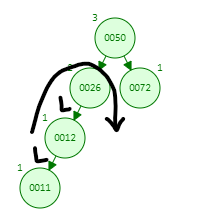
\includegraphics[width=\textwidth]{1-1-a}
        \caption{Before first rotation (LL)}
        \label{fig:1-1-a}
      \end{subfigure}
      \hfill
      \begin{subfigure}[b]{0.3\textwidth}
        \centering
        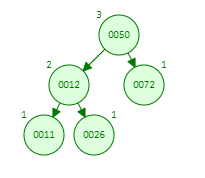
\includegraphics[width=\textwidth]{1-1-b}
        \caption{After first rotation (LL)}
        \label{fig:1-1-b}
      \end{subfigure}
      \hfill
      \begin{subfigure}[b]{0.3\textwidth}
        \centering
        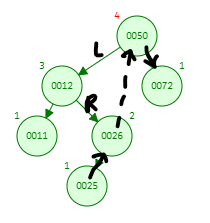
\includegraphics[width=\textwidth]{1-2-a}
        \caption{Before second rotation (LR)}
        \label{fig:1-2-a}
      \end{subfigure}
      \hfill
      \begin{subfigure}[b]{0.3\textwidth}
        \centering
        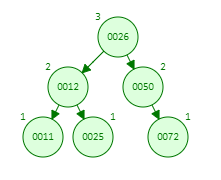
\includegraphics[width=\textwidth]{1-2-b}
        \caption{After second rotation (LR)}
        \label{fig:1-2-b}
      \end{subfigure}
      \hfill
      \begin{subfigure}[b]{0.3\textwidth}
        \centering
        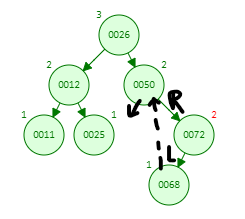
\includegraphics[width=\textwidth]{1-3-a}
        \caption{Before third rotation (RL)}
        \label{fig:1-3-a}
      \end{subfigure}
      \hfill
      \begin{subfigure}[b]{0.3\textwidth}
        \centering
        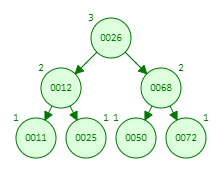
\includegraphics[width=\textwidth]{1-3-b}
        \caption{After third rotation (RL)}
        \label{fig:1-3-b}
      \end{subfigure}
      \hfill
      \begin{subfigure}[b]{0.3\textwidth}
        \centering
        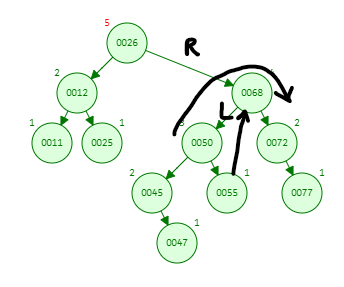
\includegraphics[width=\textwidth]{1-4-a}
        \caption{Before fourth (1st half) rotation (RL)}
        \label{fig:1-4-a}
      \end{subfigure}
      \hfill
      \begin{subfigure}[b]{0.3\textwidth}
        \centering
        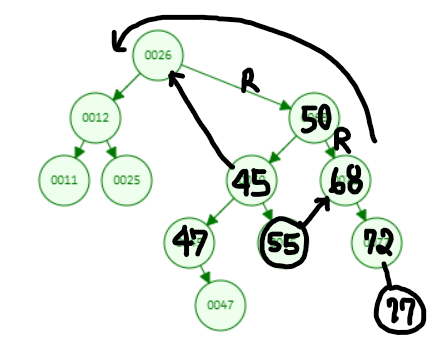
\includegraphics[width=\textwidth]{1-4-b}
        \caption{Before fourth (2nd half) rotation (RR)}
        \label{fig:1-4-b}
      \end{subfigure}
      \hfill
      \begin{subfigure}[b]{0.3\textwidth}
        \centering
        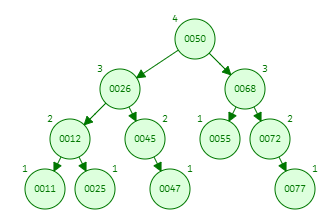
\includegraphics[width=\textwidth]{1-4-c}
        \caption{Final AVL tree}
        \label{fig:1-4-c}
      \end{subfigure}
      \caption{AVL Insertions}
      \label{fig:1}
    \end{figure}
    
    

    
    \clearpage



    \item (20 points) \textbf{Construct} a binary search tree using the following input
    (in the given order)
    \begin{equation*}
      50,\ 26,\ 72,\ 12,\ 11,\ 94,\ 53,\ 99,\ 67,\ 98,\ 37,\ 80
    \end{equation*}

    \begin{figure}[h!]
      \centering
      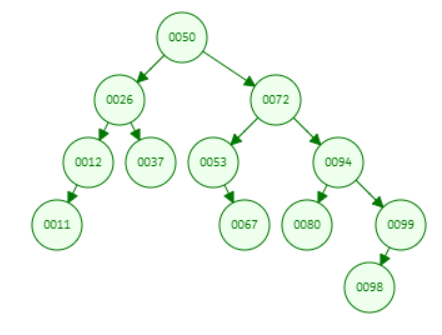
\includegraphics[width=0.25\textwidth]{2-1}
      \caption{Initial BST}
      \label{fig:2-1}
    \end{figure}

    \begin{enumerate}

      \item Is the above tree a valid AVL tree? \\
      \hspace*{\fill} \textbf{Answer:} \Highlight{No} \\
      \hspace*{\fill} \textbf{Explan.:} BF of 50 is -2
      
      \item Delete the following nodes from the above tree using the AVL
      delete (in the given order)
      \begin{equation*}
        37,\ 12,\ 80,\ 50,\ 98,\ 11
      \end{equation*}

      \textbf{Show} all your intermediate steps as you are deleting nodes from
      the tree including the rotation operations.

      \begin{figure}[h!]
        \begin{subfigure}[b]{0.3\textwidth}
          \centering
          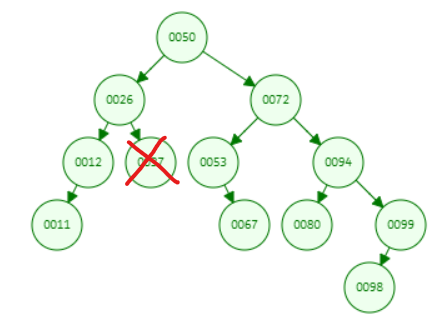
\includegraphics[width=\textwidth]{2-2-a}
          \caption{Deleting 37}
          \label{fig:2-2-a}
        \end{subfigure}
        \hfill
        \begin{subfigure}[b]{0.3\textwidth}
          \centering
          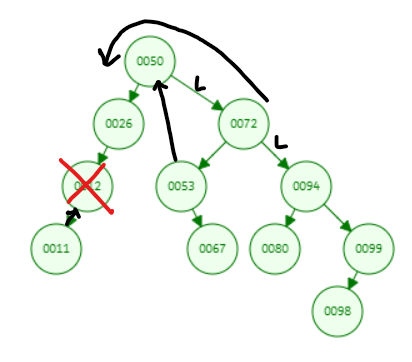
\includegraphics[width=\textwidth]{2-2-b}
          \caption{Deleting 12; before LL rotation}
          \label{fig:2-2-b}
        \end{subfigure}
        \hfill
        \begin{subfigure}[b]{0.3\textwidth}
          \centering
          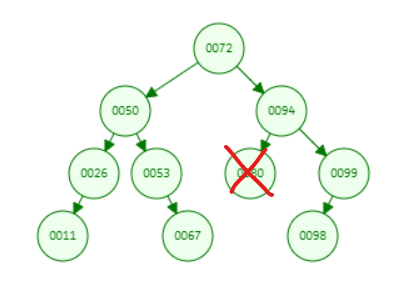
\includegraphics[width=\textwidth]{2-2-c}
          \caption{Deleting 80; after LL rotation}
          \label{fig:2-2-c}
        \end{subfigure}
        \hfill
        \begin{subfigure}[b]{0.3\textwidth}
          \centering
          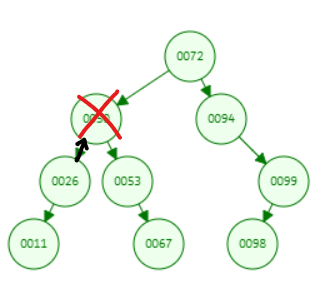
\includegraphics[width=\textwidth]{2-2-d}
          \caption{Deleting 50; replace with predecessor}
          \label{fig:2-2-d}
        \end{subfigure}
        \hfill
        \begin{subfigure}[b]{0.3\textwidth}
          \centering
          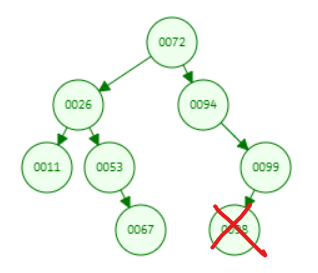
\includegraphics[width=\textwidth]{2-2-e}
          \caption{Deleting 98}
          \label{fig:2-2-e}
        \end{subfigure}
        \hfill
        \begin{subfigure}[b]{0.3\textwidth}
          \centering
          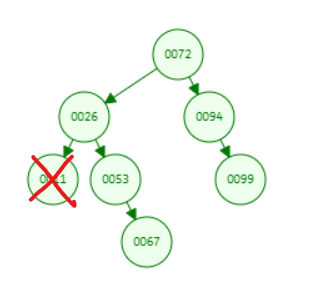
\includegraphics[width=\textwidth]{2-2-f}
          \caption{Deleting 11}
          \label{fig:2-2-f}
        \end{subfigure}
        \hfill
        \begin{subfigure}[c]{0.3\textwidth}
          \centering
          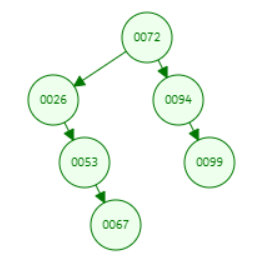
\includegraphics[width=\textwidth]{2-2-g}
          \caption{Final AVL tree}
          \label{fig:2-2-g}
        \end{subfigure}
        \caption{AVL Deletions}
        \label{fig:2}
      \end{figure}

    \end{enumerate}



    \clearpage



    \item (20 points) \textbf{Construct} a red-black tree using the following input (in
    the given order)
    \begin{equation*}
      50,\ 26,\ 72,\ 37,\ 28,\ 15,\ 17,\ 24
    \end{equation*}

    \textbf{Show} all your intermediate steps including the recoloring and restruc-
    turing operations.

    \textit{Note:} nodes circled in red mean red nodes, in black means black nodes, regardless of node text or background color.

    \begin{figure}[h!]
      \begin{subfigure}[b]{0.3\textwidth}
        \centering
        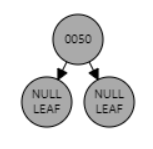
\includegraphics[width=\textwidth]{3-1-a}
        \caption{Inserted 50}
        \label{fig:3-1-a}
      \end{subfigure}
      \hfill
      \begin{subfigure}[b]{0.3\textwidth}
        \centering
        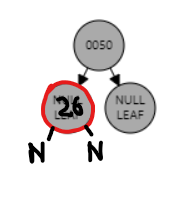
\includegraphics[width=\textwidth]{3-1-b}
        \caption{Inserting 26}
        \label{fig:3-1-b}
      \end{subfigure}
      \hfill
      \begin{subfigure}[b]{0.3\textwidth}
        \centering
        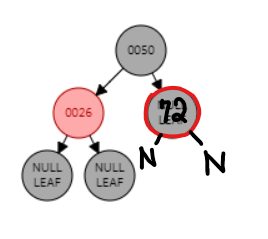
\includegraphics[width=\textwidth]{3-1-c}
        \caption{Inserting 72}
        \label{fig:3-1-c}
      \end{subfigure}
      \hfill
      \begin{subfigure}[b]{0.3\textwidth}
        \centering
        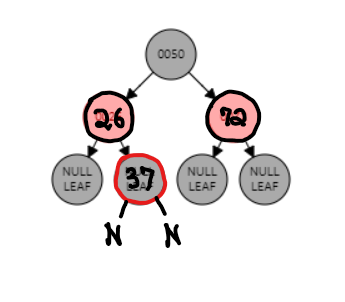
\includegraphics[width=\textwidth]{3-1-d}
        \caption{Inserting 37; recoloring children of 50}
        \label{fig:3-1-d}
      \end{subfigure}
      \hfill
      \begin{subfigure}[b]{0.3\textwidth}
        \centering
        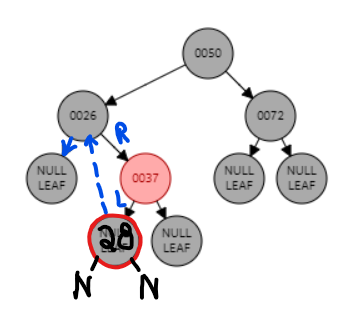
\includegraphics[width=\textwidth]{3-2-a}
        \caption{Inserting 28; before RL rotation and recoloring}
        \label{fig:3-2-a}
      \end{subfigure}
      \hfill
      \begin{subfigure}[b]{0.3\textwidth}
        \centering
        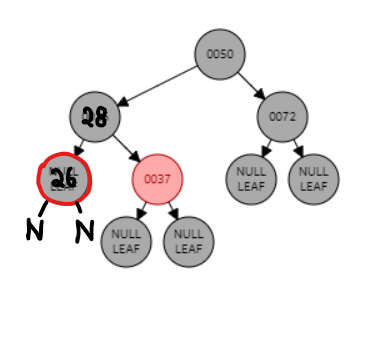
\includegraphics[width=\textwidth]{3-2-b}
        \caption{Inserting 28; after RL rotation and recoloring}
        \label{fig:3-2-b}
      \end{subfigure}
      \hfill
      \begin{subfigure}[b]{0.3\textwidth}
        \centering
        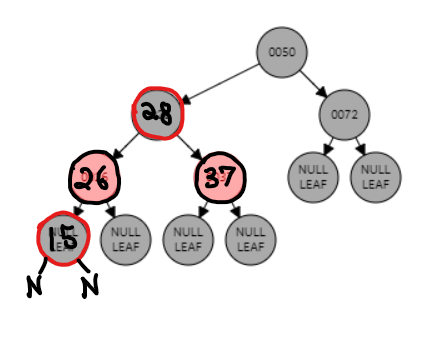
\includegraphics[width=\textwidth]{3-2-c}
        \caption{Inserting 15; recoloring 28 and its children}
        \label{fig:3-2-c}
      \end{subfigure}
      \hfill
      \begin{subfigure}[b]{0.3\textwidth}
        \centering
        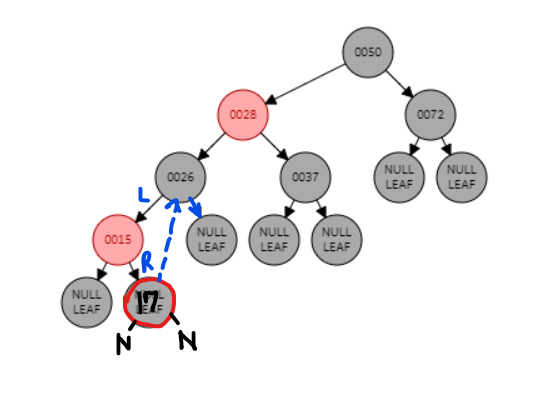
\includegraphics[width=\textwidth]{3-3-a}
        \caption{Inserting 17; before LR rotation and recoloring}
        \label{fig:3-3-a}
      \end{subfigure}
      \hfill
      \begin{subfigure}[b]{0.3\textwidth}
        \centering
        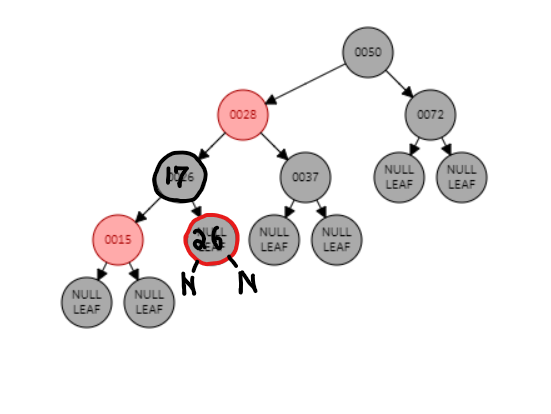
\includegraphics[width=\textwidth]{3-3-b}
        \caption{Inserting 17; after LR rotation and recoloring}
        \label{fig:3-3-b}
      \end{subfigure}
      \hfill
      \begin{subfigure}[b]{0.3\textwidth}
        \centering
        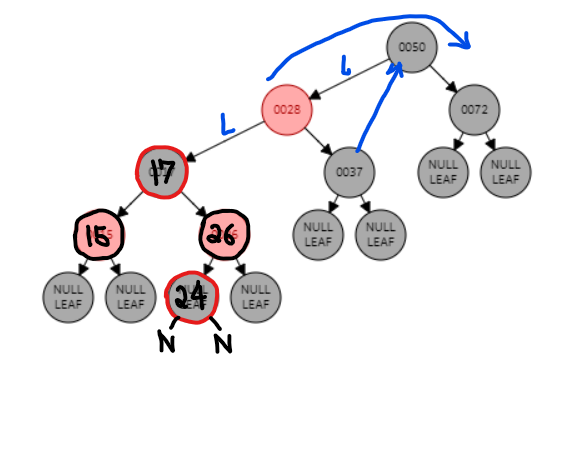
\includegraphics[width=\textwidth]{3-4-a}
        \caption{Inserting 24; recoloring 17 and its children; before LL rotation}
        \label{fig:3-4-a}
      \end{subfigure}
      \hfill
      \begin{subfigure}[b]{0.3\textwidth}
        \centering
        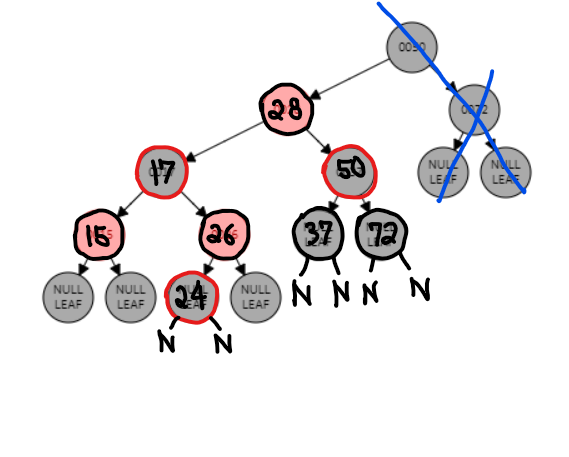
\includegraphics[width=\textwidth]{3-4-b}
        \caption{Inserting 24; after LL rotation and recoloring}
        \label{fig:3-4-b}
      \end{subfigure}
      \hfill
      \begin{subfigure}[b]{0.3\textwidth}
        \centering
        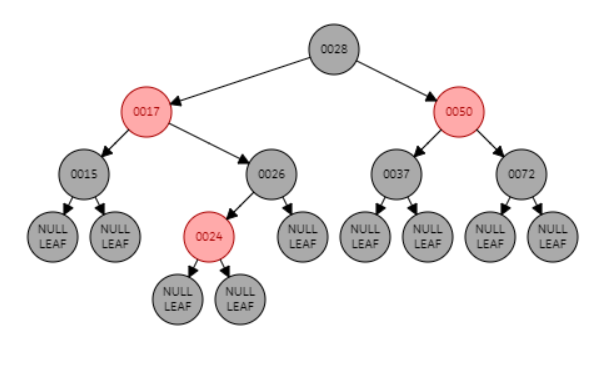
\includegraphics[width=\textwidth]{3-4-c}
        \caption{Final red-black tree}
        \label{fig:3-4-c}
      \end{subfigure}
      \caption{RBT Insertions}
      \label{fig:3}
    \end{figure}

\end{enumerate}

\end{document}

% TK TODO
% - relabel to RR in figure 8 before fourth (2nd half) rotation (LL->RR)
% - fix positioning of figures
% - condense figures into subfigures